\documentclass[Rapport/Rapport_main.tex]{subfiles}
\begin{document}
\subsection{BallCountSensor}\label{sec:BallCountSensor}
Denne sensor står for at notificere systemet om hvor vidt bolddispenseren har brug for flere bolde.

\paragraph{Harware Design}
\newline\newline
Det var klart i begyndelsen af design at dette skulle være en lyssensor. Boldene vejer for lidt til en pålidelig måling, og en kapacitans sensor er ikke praktisk i forhold til bolddispenserens fysiske dimensioner. Desuden er der meget mørk i bolddispenseren så en lyssensor vil ikke blive forstyrret. I starten var det to lyssensorer der skulle placeres på bolddispenseren. En i top og en i bunden, til at måle henholdsvis en fyldt op tilstand og tom tilstand. Det var dog mere interesant og kompakt at bruge kun én lyssensor, som kunne måle afstande. På den måde kan man skrive et program der holder styr på afstanden og oversætter denne til et bestemt antal bolde.//

Der valges at lave et lyssensor der kan måle afstand. For at undgå forstyringer under genopfyldningen af bolddispenseren, laves der et låg i toppen af bolddispenser beholderen hvor sensoren kan sidde.//

Der bruges en IR-emitter (SFH485) og en fotodiode (SFH203FA) til afstands sensoren. Det undersøges hvordan fotodioden og IR-emitteren fungerer. Ind i datasheet for fotodioden står der en fotostrøm, som bliver genereret af fotodioden når den får infrarød lys. I dette design er IR-emitterens opgave er at blinke ind bolddispenserens beholder så dens lys kan blive reflekteret af de bolde der er. Fotodioden skal vha. sin revers bias strøm oplyse os om hvor langt væk det først bold ramt af emitteren er, og dermed hvor mange bolde der er tilbage. Da fotodiodens revers bias strøm er afhængig af det effekt densitet som infrarødlys giver ($mW/cm^2$), så regnes der ikke med en lineær sammenhæng mellem afstand og fotostrøm.
Der ventes med at tests, da forholdene ind i bolddispenseren er væsentlig anderledes end udenfor. Derfor afvikles der et kredsløb som nemt kan re-dimensioneres efter behov. Det skal sikres ,at sensoren kan måle forholdsvis store afstande. Derfor er en stærk lysintensitet ud af IR-emitter vigtigt.//
IR-emitter lyser stærkest alt efter hvor meget strøm den forsynes med, men den bliver også varmere, dette giver anledning til et klasisk switch-kredsløb, så IR-emitteren ikke er tændt konstant. Vi kigger på datasheet og finder en graf for pulsevne, her aflæses at IR-emitteren kan tåle $300mA$ i $500\mu s$ med en pulsbredde på $0.2$. Vi beregner vores pulsfrekvens til:
\[\frac{0.2}{500\mu s}=400Hz\]
En npn-transistor ville være ideelt til at slukke og tænde for strøm. Der søges efter en transistor der både kan levere det strøm i collector og kan switche hurtigt nok. Her vælges BC517 darlington NPN transistor da denne kan levere op til 500mA og behøver ikke en stor base strøm. Der sættes resistor ved base og collector for at styr strømmen gennem IR-led og strømmen ind i basen. Opstilling ses på figur \ref{fig:IRLEDpuls}.
\begin{figure}[H]
    \centering
    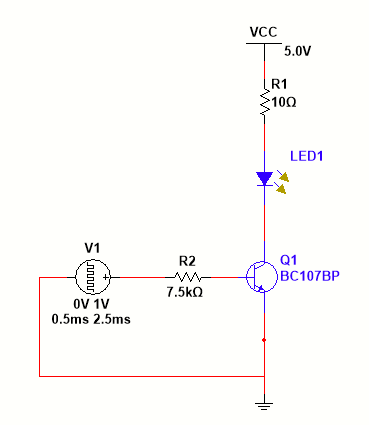
\includegraphics{Rapport/BallDispenser/BallCountSensor/graphics/Opstilling1.png}
    \caption{Opstilling for at pulse med IR-LED}
    \label{fig:IRLEDpuls}
\end{figure}

Nu at vi har vores blinkende infrarød emitter er vi nødt til at finde en måde at detektere refleksionerne med fotodioden. Her bruges 4 komponenter: En modstand, en sample-hold kredsløb, en ADC-konverter og en PWM generator. Modstanden bruges til at forstærke signalet, som så samples af sample-hold kredsløbet. ADC-konverteren er vigtigt da den oversætter vores spændingsværdi til et tal som kan bruges.
Vi benytter at $U=R\cdot I$, det betyder at hvis vi gerne vil detektere en lille strøm i form af en spænding, så har vi brug for en stor modstand. Derfor bruges der en $1M\Omega$ modstand. Et andet mulighed, var at bruge en transimpedans operatinsforstærker, som der bruges i Cup Sensor. Opstillingen for fotodioden er meget enkelt og kan ses på figur \ref{fig:fotodiode_opstilling}.
\begin{figure}[H]
    \centering
    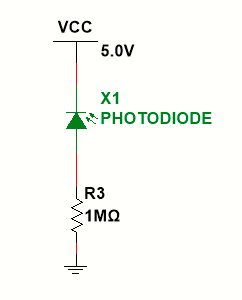
\includegraphics{Rapport/BallDispenser/BallCountSensor/graphics/Opstilling1_2.png}
    \caption{Opstilling for fotodiode}
    \label{fig:fotodiode_opstilling}
\end{figure}
Da vi pulser med IR-LED, kan vi ikke regne med et konstant spænding over modstanden i figur \ref{fig:fotodiode_opstilling}. Vi vil gerne have en konstant spænding fordi det er nemmere at arbejde med, og fordi spænding skal være et udtryk for hvormange bolde der. Det er her sample-hold komponenten i PSoC er nyttigt. Som navnet siger, så samples der en spænding på et givet tidspunkt, og denne spænding holdes, indtil næste sampling. Det eneste vi skal sørge for, er at timingen mellem IR-LED pulse og sampling er optimalt. Det er klart at både IR-LED transistor i figur 1.1 og samplehold komponenten skal drives af samme PWM signal, sådan så når IR-LED blinker, så samples der en spænding foran fotodioden. Opstilling kan ses på  figur \ref{fig:PSoC_TopDesign}.
\begin{figure}[H]
    \centering
    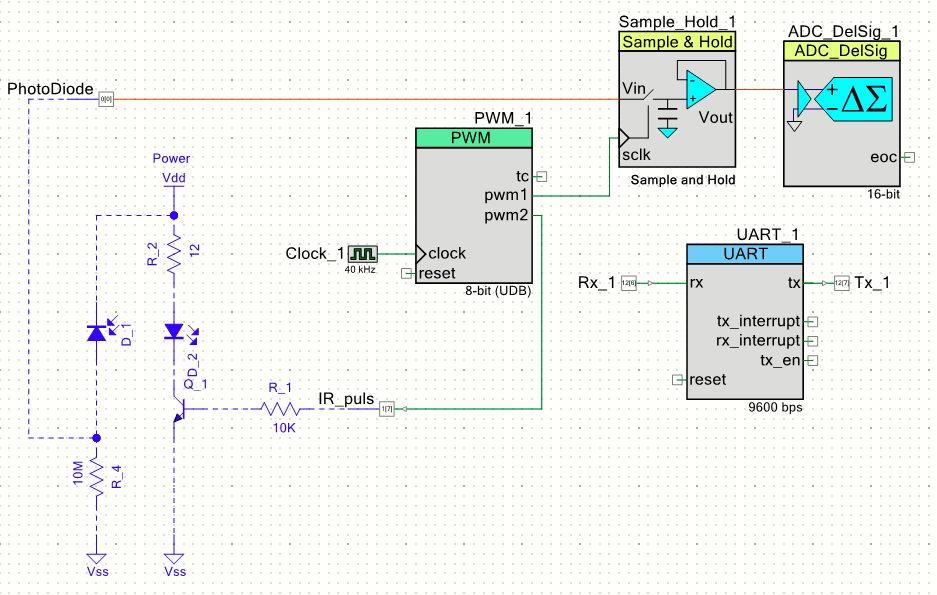
\includegraphics[width=1\textwidth]{Rapport/BallDispenser/BallCountSensor/graphics/Opstilling2.png}
    \caption{Opstilling for Ball Count sensor kredsløb}
    \label{fig:PSoC_TopDesign}
\end{figure}

\paragraph{Målinger og kalibrering}
\newline
\newline
Før vi implementere kredsløbet sammen med PSoC er det en god ide at lave nogle målinger af vores IR-LED strøm og fotodiode spænding. Her laves kredsløbene fra figur figur \ref{fig:IRLEDpuls} og \ref{fig:fotodiode_opstilling} på fumlebræt og Analog Discovery og en power-supply fra lab bruges i stedet for PSoC til at drive og måle på kredsløbet. Vi måler først spændingen generet af fotodiodens reverse-biased strøm. Spændingen måles mellem modstanden R3 og fotodioden (figur \ref{fig:fotodiode_opstilling}). Ved alle målinger pulser vi med 400Hz med en pulsebredde på 20\%.
\begin{figure}[H]
    \centering
    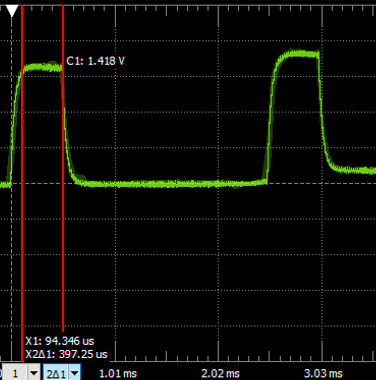
\includegraphics{Rapport/BallDispenser/BallCountSensor/graphics/Maling1.png}
    \caption{Måling af spændings rise-time ved fotodiodens modstand}
    \label{fig:Måling1_AD}
\end{figure}
På målingen i figur \ref{fig:Måling1_AD} kan man se, at spændingen genereret af fotodiodens strøm gennem en stor modstand, efterligner den pulse-signal som IR-LED drives med. Det vil sige vores koncept for hele sensoren gælder. Vi observere også, at denne spænding tager lidt længere tid om at komme op på et dc-niveau. Vi skal derfor ændre vores valg om at sample samtidigt med at vi pulser. Målingen viser et dc-niveau i en pulsebredde med en tid på $397\mu s$ og en frekvens på 400Hz. Derfor må vi antage at sensor kan ses som et PWM signal på 400Hz med en pulsbredde på 15.9\%. Det beregnes således.
$$400Hz\cdot 397\mu s=0.159\%$$
For at være på den sikre side vælger vi at sample med 400 Hz og en pulsbredde på 14\%. Kalibrering på PSoC kan ses på figur \ref{fig:PWM_timing}.
\begin{figure}[H]
    \centering
    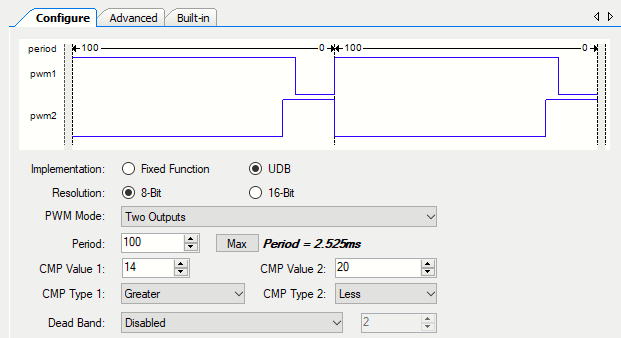
\includegraphics[width=1\textwidth]{Rapport/BallDispenser/BallCountSensor/graphics/PWM_timing.png}
    \caption{PWM signal pulsbredde timing}
    \label{fig:PWM_timing}
\end{figure}
Der gøres opmærksom på at Sample-Hold komponenten i PSoC sampler ved falling-edge. Næst måles strømmen gennem IR-LED, ved at måle spændingsfaldet over formodstanden R1 fra opstillingen i figur \ref{fig:IRLEDpuls}.
\begin{figure}[H]
    \centering
    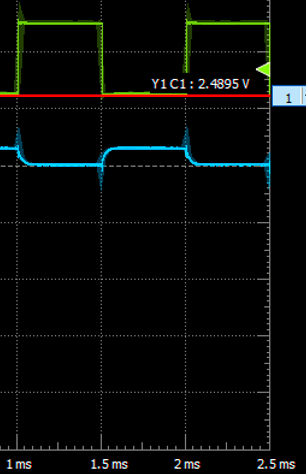
\includegraphics[width=0.27\textwidth]{Rapport/BallDispenser/BallCountSensor/graphics/Maling2.png}
    \caption{Måling af strøm gennem IR-LED}
    \label{fig:Måling2_AD}
\end{figure}
Her bergnes strømmen til 
$$\frac{(5-2.49)V}{10\Omega}=251mA$$
Her kalibreres ved at ændre på modstanden, så strømmen er lidt højere. Her vælger vi en modstand på $8.2\Omega$ som giver os en strøm på 306mA.
Kredsløbet er klar til at sættes sammen med PSoC. Opstillingen forbliver den samme som på figur \ref{fig:PSoC_TopDesign}. Hvor R2 er ændret til $8\Omega$ og R1 til $7.5k\Omega$
Ind i koden for PSoC bruger vi UART og ADC til at måle værdier alt efter hvormange bolde der i cylingerbeholderen. Et billede af denne måle opstilling kan ses på figur(????).
\end{document}